\documentclass[letterpaper,11pt]{article}

\usepackage{amsmath}
\usepackage{amssymb}
\usepackage[hmargin=1.25in,vmargin=1in]{geometry}
\usepackage{graphicx}
\usepackage{hyperref}
\usepackage{listings}
\usepackage{lmodern}
\usepackage{microtype}
\usepackage{minted}

\DeclareMathOperator*{\argmin}{arg\,min}

\author{Philip Pham}
\date{\today}
\title{CSE 547 - Assignment 1}

\begin{document}
\maketitle

\section*{Problem 0}

\begin{description}
\item[List of collaborators:] I have not collaborated with anyone.
\item[List of acknowledgements:] None.
\item[Certify that you have read the instructions:] Yes.
\item[Terms and Conditions to use the dataset:] I accept the terms and
  conditions to use the COCO dataset.
\end{description}

\section*{Problem 1}

Read the course website, up until ``Lecture Notes and Readings'', so that you
understand the course policies on grading, late policies, projects, requirements
to pass etc. Write ``I have read and understood these policies'' to certify
this. If you have questions, please contact the instructors.

\subsection*{Solution}

I have read and understood these policies.

\section*{Problem 2}

Consider the function from class (and the notes):
\begin{equation}
  f\left(w_1,w_2\right) = \left[\sin\left(2\pi\frac{w_1}{w_2}\right) + 3\frac{w_1}{w_2} - \exp\left(2w_2\right)\right]\left[3\frac{w_1}{w_2} - \exp\left(2w_2\right)\right].
\end{equation}

Suppose our program for this function uses the following evaluation trace:

\begin{description}
\item[input:] $z_0 = \left(w_1,w_2\right)$
  \begin{enumerate}
  \item $z_1 = w_1/w_2$
  \item $z_2 = \sin\left(2\pi z_1\right)$
  \item $z_3 = \exp\left(2w_2\right)$
  \item $z_4 = 3z_1 - z_3$
  \item $z_5 = z_2 + z_4$
  \item $z_6 = z_4z_5$
  \end{enumerate}
\item[return:] $z_6$
\end{description}

\subsection*{The Forward Mode of AutoDiff (AD)}

The forward mode for auto-differentiation is a conceptually simpler
way to compute the derivative. Let us examine the forward mode to
compute the derivative of one variable, $\frac{df}{dw_1}$. In the
forward mode, we sequentially compute both $z_t$ and its derviative
$\frac{dz_t}{dw_1}$ using the previous variables $z_1,\ldots,z_{t-1}$
and the previous derivatives
$\frac{dz_1}{dw_1},\ldots,\frac{dz_{t-1}}{dw_1}$.

Explicitly write out the forward mode in our example.

\subsubsection*{Solution}

In the forward mode, we sequentially compute the values $z_t$ and derivates of
$z_t$ with respect to $w_1$ in order for $t = 1,2,\ldots,6$.

Suppose we want to calculate $\frac{df}{dw_1}(u,v)$. Fix $w_1 = u$ and
$w_2 = v$.

\begin{enumerate}
\item Compute $z_1 = u/v$.
\item Compute $\frac{dz_1}{w_1} = 1/v$.
\item Compute $z_2 = \sin\left(2\pi z_1\right)$.
\item Compute
  $\displaystyle\frac{dz_2}{dw_1} = \frac{\partial z_2}{\partial
    z_1}\frac{dz_1}{w_1} = 2\pi\cos\left(2\pi z_1\right)\frac{dz_1}{w_1}$.
\item Compute $z_3 = \exp\left(2v\right)$.
\item Compute $\displaystyle \frac{dz_3}{dw_1} = 0$.
\item Compute $z_4 = 3z_1 - z_3$.
\item Compute
  $\displaystyle \frac{dz_4}{dw_1}= \frac{\partial z_4}{\partial z_1}\frac{dz_1}{dw_1} + \frac{\partial z_4}{\partial z_3}\frac{dz_3}{dw_1} = 3\frac{dz_1}{dw_1} - \frac{dz_3}{dw_1}$.
\item Compute $z_5 = z_2 + z_4$.
\item Compute $\displaystyle \frac{dz_5}{dw_1} = \frac{\partial z_5}{\partial z_2}\frac{dz_2}{dw_1} + \frac{\partial z_5}{\partial z_4}\frac{dz_4}{dw_1} = \frac{dz_2}{dw_1} + \frac{dz_4}{dw_1}$.
\item Compute $z_6 = z_4z_5$.
\item Compute $\displaystyle\frac{dz_6}{dw_1} = \frac{\partial z_6}{\partial z_4}\frac{dz_4}{dw_1} + \frac{\partial z_6}{\partial z_5}\frac{dz_5}{dw_1} = z_5\frac{dz_4}{dw_1} + z_4\frac{dz_5}{dw_1}$.
\end{enumerate}

Each step can be computed by substituting values from the previous steps. The
output is $\displaystyle\boxed{\frac{df}{dw_1}(u,v) = \frac{dz_6}{dw_1}.}$

\subsection*{The reverse mode of AD}

Now let use consider the reverse mode to compute the derivative
$\frac{df}{dw}$, which is a two-dimensional vector.

Explicitly write out the reverse mode in our example with the assumption that
you have evaluated the trace and already stored all the $z_t$s in memory
already.

\subsubsection*{Solution}

In the reverse mode, we compute $\frac{df}{dz_t} = \frac{dz_6}{dz_t}$ in order
$t = 6,5,\ldots,0$. The general algorithm is
\begin{equation}
  \frac{dz_6}{dz_t} = \sum_{\text{$c$ is a child of $t$}}
  \frac{dz_6}{dz_c}
  \frac{\partial z_c}{\partial z_t}.
\end{equation}

\begin{enumerate}
\item Seed $\displaystyle \frac{dz_6}{dz_6} = 1$.
\item Compute
  $\displaystyle \frac{dz_6}{dz_5} =
  \frac{dz_6}{dz_6}\frac{\partial z_6}{\partial z_5} = z_4$.
\item Compute
  $\displaystyle \frac{dz_6}{dz_4} = \frac{dz_6}{d z_5}\frac{\partial
    z_5}{\partial z_4} + \frac{d z_6}{d z_6}\frac{\partial z_6}{\partial z_4} =
  \frac{dz_6}{d z_5} + \frac{d z_6}{d z_6}z_5
  =
  z_4 + z_5
  $.
\item Compute
  $\displaystyle \frac{dz_6}{dz_3} = \frac{dz_6}{d z_4}\frac{\partial
    z_4}{\partial z_3} = -\frac{dz_6}{d z_4} = -z_4 - z_5$.
\item Compute
  $\displaystyle \frac{dz_6}{dz_2} = \frac{dz_6}{d z_5}\frac{\partial
    z_5}{\partial z_2} = \frac{dz_6}{d z_5} = z_4$.
\item Compute
  $\displaystyle \frac{dz_6}{dz_1} =
  \frac{dz_6}{d z_2}\frac{\partial  z_2}{\partial z_1} +
  \frac{dz_6}{d z_4}\frac{\partial  z_4}{\partial z_1} =
  2\pi\cos\left(2\pi z_1\right)\frac{dz_6}{d z_2} +
  3\frac{dz_6}{d z_4}$.
\item Compute
  $\displaystyle
  \frac{dz_6}{dw_1} = \frac{dz_6}{dz_1}\frac{\partial z_2}{\partial w_1}
  = \frac{1}{w_2}\frac{dz_6}{dz_1}$.
\item Compute
  $\displaystyle
  \frac{dz_6}{dw_2} = \frac{dz_6}{dz_1}\frac{\partial z_1}{\partial w_2} +
  \frac{dz_6}{dz_3}\frac{\partial z_3}{\partial w_2}
  = -\frac{w_1}{w_2^2}\frac{dz_6}{dz_1} + 2\exp\left(2w_2\right)\frac{dz_6}{dz_3}$.
\end{enumerate}

Each step can be computed by substituting the output of one of the previous
steps. From the last two steps, we obtain our desired result
\begin{equation}
  \boxed{
    \frac{df}{dw} = \begin{pmatrix}
      \displaystyle\frac{dz_6}{dw_1} \\ \displaystyle\frac{dz_6}{dw_2}
    \end{pmatrix}.
  }
\end{equation}

\section*{Problem 3: Computation and Memory in AD}

Suppose we seek to compute the derivative with respect to a real valued function
$f\left(w\right) : \mathbb{R}^d \rightarrow \mathbb{R}$. Let us examine some of
the computational and memory issues involved in AD.

\subsection*{Computation}

Let $T$ be the computation time to compute $f(w)$ using our program.

\begin{enumerate}
\item Suppose we want to find the derivative of one variable $\frac{df(w)}{dw_1}$
  with respect to the variable $w_1$. In order notation, how does the
  computational complexity (the runtime) of the forward mode compare to the
  reverse mode $\frac{df(w)}{dw_1}$?
  \subsubsection*{Solution}

  For the forward mode, we just do one sweep through our computation graph to
  compute $\frac{df(w)}{dw_1}$, so the running time is $O(T)$.

  In the reverse mode, we also just do one sweep through the graph, so the
  running time is also $O(T)$.

  Both running times are of the same complexity in this case.
  
\item Suppose we want to find the derivative $\frac{df(w)}{dw}$,which is a
  $d$-dimensional vector. How would we do this with the forward mode and, in
  order notation, what is the computational complexity? Again, in order
  notation, how does the computational complexity (the runtime) of the forward
  mode compare to the reverse mode to compute $\frac{df(w)}{dw}$.
  \subsubsection*{Solution}

  For the forward mode, we have to do a sweep for each
  $\frac{df(w)}{dw_1},\ldots,\frac{df(w)}{dw_d}$ that we want to compute, so the
  runtime complexity is $O(Td)$.

  In the reverse mode, we have to do one sweep. Then, we have enough
  information to compute each $\frac{df(w)}{dw_j}$, so the runtime complexity is
  $O(T + d)$.

  The computational complexity of the reverse mode is smaller than that of the
  forward mode.
  
  \item If we could easily parallelize our computation (not worrying about
    communication), do you see a way to speed up the reverse mode? If so, what
    would be the new serial runtime? If not, why?
    \subsubsection*{Solution}

    Only one sweep needs to be done, and sweeping though the graph must be done
    in a certain order, so there is no easy way to parallelize that part. Once
    the sweep is done, one could use the computed intermediate derivatives to to
    calculate each $\frac{df(w)}{dw_j}$ in a parallel manner. In that case the
    new runtime complexity is $O(T)$.
    
  \item If we could easily parallelize our computation (not worrying about
    communication), do you see a way to speed up the forward mode? If so, how so
    and what would be the new serial runtime? If not, why?
    \subsubsection*{Solution}

    Yes. The obvious way is to parallize the forward mode is to have $d$ workers
    each doing a separate sweep and computing a separate
    $\frac{df(w)}{dw_j}$. If we do that, the runtime complexity is also $O(T)$.
\end{enumerate}

\subsection*{Memory}

Memory is often a bottleneck in practice (e.g. we load as much as we can on a
GPU when doing our computation in batches of data). Let us understand some of
these issues.  Suppose our input $w$ is $d$-dimensional and our evaluation trace
is $T$ steps. Assume one unit of memory is required to store a real
number. Also, assume that we are free to delete variables at any time to free up
memory (in practice, this often occurs by overwriting variables).  In this
question, when memory is used to refer to how much ``scratch space'' we need to
utilize in order to run our program. In this question, order notation is
sufficient. When stating your answers do not include the memory required to
store the parameter $w$ or the program itself. Also, when in your answers, do
not include the memory required to write out the programs output (assume we have
already allocated this memory). We are interested in how much excess memory the
program needs to have free in order to store its intermediate variables and do
all its computations.

\begin{enumerate}
\item Suppose that we were just interested in computing $f(w)$. Is it often the
  case that we can get away with less than $T$ units of memory? How so?

  \subsection*{Solution}
  Yes, we can get away with less than $T$ units of memory by discarding
  unnecessary intermediate variables. 

  For example suppose the computation graph was a perfectly balanced tree and
  $z_T = z_{T - 1} + z_{T-2}$ where the computation traces of
  $z_{T - 1} + z_{T-2}$ are each $(T - 1)/2$. After computing $z_{T - 1}$, we
  can free any memory used to compute it.
  
\item Suppose we only need to use $m$ units of memory to compute $f(w)$. If we
  only wanted to compute $\frac{df}{dw_1}$, how much memory would we require to
  compute this using the forward mode? Explain.

  \subsection*{Solution}
  We also only need $O(m)$ units of memory to compute $\frac{df}{dw_1}$. Suppose
  that we are trying to compute $z_t$. We only need to know the value of its
  parents. To compute $\frac{dz_t}{dw_1}$, we only need to know the value of its
  parents and the derivatives of the of the parents with respect to $w_1$.
\item Suppose we only need to use $m$ units of memory to compute $f(w)$. If we
  only wanted to compute $\frac{df}{dw_1}$, how much memory would we require to
  compute this using the reverse mode? Explain.

  \subsection*{Solution}

  Since we want to avoid blowing up the computation, we need $O(T)$ units of
  memory. One may think that since the computation of $\frac{dz_T}{dz_t}$ only
  requires the children of $z_t$, less units of memory are needed. But since
  we're working backwards, we may be deep in the graph, so those children have
  to be computed ahead of time. The first steps require knowing the values near
  the leaves for instance. If we discarded the intermediate values, we would may
  to do expensive calculations to recover them when deep in the graph.

\item Suppose we only need to use $m$ units of memory to compute $f(w)$ and
  suppose we want to compute $\frac{df}{dw}$. If we don't care about runtime,
  what is the most memory efficient algorithm you can come up with? How much
  memory is needed?

  \subsection*{Solution}

  We could just repeat the forward pass to compute each $\frac{df}{dw_j}$. Each
  pass takes $O(m)$. After we're done the pass, we would discard any
  intermediate variables and just keep $\frac{df}{dw_j}$. If $w$ is
  $d$-dimensional, we only need $O(m + d)$ units of memory.
  
\end{enumerate}

\section*{Problem 4: PyTorch Can Give Us Some Crazy Answers}

Now you will construct an example in which PyTorch provides derivatives that
make no sense. The issue is in understanding when it is ok and when it is not ok
to use dynamic computation graphs. You are going to find a way code up the same
function in two different ways so that PyTorch will return different derivatives
at the same point. The purpose of this exercise is to better understand how
dynamic computation graphs work and to understand what you are doing when you
using various AD softwares.

\subsection*{Two Identical Non-differentiable Functions with Different ``Derivatives''}

\begin{enumerate}
\item Define \emph{and} plot a one dimensional, real valued function
  which is not continuous.
  
  \subsubsection*{Solution}
  Consider the function
  \begin{equation}
    f(x) = \begin{cases}
      2x, - 1& x < 0; \\
      0, & x = 0; \\
      2x + 1, & x > 0.
    \end{cases}
    \label{eqn:problem4}
  \end{equation}

  It is implemented in Listings \ref{lst:f} and \ref{lst:g} and plotted in
  Figure \ref{fig:problem4}.

  \begin{figure}[h]
    \centering
    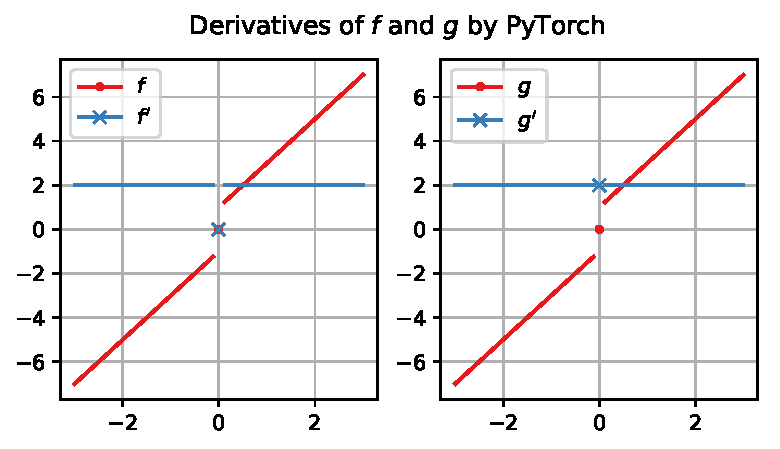
\includegraphics{problem4/problem4.pdf}
    \caption{The functions from Listings \ref{lst:f} and \ref{lst:g} are plotted
      along with their PyTorch-computed derivatives.}
    \label{fig:problem4}
  \end{figure}
\item Now write out your function in PyTorch. You should be able to
  define this function so that PyTorch returns a derivative of $0$ at
  some point $x_0$.
  \subsubsection*{Solution}
  Equation \ref{eqn:problem4} is implemented as $f$ in Listing
  \ref{lst:f}. In Figure \ref{fig:problem4}, you can see that PyTorch
  calculates the derivative as $0$ at $x_0 = 0$ (left plot, blue
  \texttt{x}).
  
  \begin{listing}
\begin{minted}{python}
def f(x: Variable) -> Variable:
    assert x.requires_grad
    return (2*x*torch.sign(x) + 1)*torch.sign(x)
\end{minted}
  \caption{Equation \ref{eqn:problem4} defined with the sign function factored out.}
\label{lst:f}
\end{listing}

\item Now find another way to write out your function in PyTorch; do
  this so that it is exactly the same function. Do this in a way so
  that PyTorch now returns a derivative of $2$ at exactly the same
  point $x_0$ that you obtained a derivative of $0$ in the previous
  question.
  \subsubsection*{Solution}
  Equation \ref{eqn:problem4} is implemented as $g$ in Listing
  \ref{lst:g}. In Figure \ref{fig:problem4}, you can see that PyTorch
  calculates the derivative as $2$ at $x_0 = 0$ (right plot, blue
  \texttt{x}).
  
\begin{listing}
\begin{minted}{python}
def g(x: Variable) -> Variable:
    def g1d(x: Variable) -> Variable:
        if x.data[0] > 0:
            return 2*x + 1
        elif x.data[0] < 0:
            return 2*x - 1
        else:
            return 2*x

    if x.dim() == 0:
        return 1*x    
    if x.size() == torch.Size([1]):
        return g1d(x)

    return torch.stack([g(sub_x) for sub_x in x])
\end{minted}
  \caption{Equation \ref{eqn:problem4} defined element-wise by recursing into the tensor.}
\label{lst:g}
\end{listing}
\item There is a no sane definition of the derivative for your
  function. Yet, you should not only found a way to get PyTorch to
  provide a derivative, you should have also found a way to give you
  two \emph{different} derivatives at exactly the same point (on the same
  function). What went wrong?

  \subsubsection*{Solution}

  PyTorch is just keeping track of the operations and does a pointwise
  calculation. It's not paying attention to any local behvaior like
  continuity. In Listing \ref{lst:g}, by changing the \texttt{else}
  arm, we can have it return any arbitrary number for the
  derivative. For instance, having it return \texttt{-3*x} would have
  PyTorch calculating the derivative as $-3$ at $x_0 = 0$.
\end{enumerate}

\subsection*{Extra Credit: Differentiable Functions with Different ``Derivatives''}

Provide a differentiable function, where you can code it up in PyTorch
in two different ways and where you can get two different derivatives
at the same point $x_0$.

\subsubsection*{Solution}

We can reuse the same idea. PyTorch doesn't correctly compute the
derivative when squaring the sign function, even though, the sign
function squared is just the identity.

Using this, I implement the simple, differentiable line $f(x) = 2x$ in
two ways: (1) verbosely using the sign function as $f$ and (2) the
canonical way as $g$ in Listing \ref{lst:fg_diff}.

\begin{listing}
\begin{minted}{python}
def f(x: Variable) -> Variable:
    assert x.requires_grad
    return 2*x*torch.sign(x)*torch.sign(x)

def g(x: Variable) -> Variable:
    assert x.requires_grad
    return 2*x
\end{minted}
  \caption{The function $f(x) = 2x$ defined in two different ways.}
\label{lst:fg_diff}
\end{listing}

This results in Figure \ref{fig:problem4_differentiable}. PyTorch
computes $f^\prime(0) = 0$ despite the true value being $2$.

\begin{figure}[h]
  \centering
  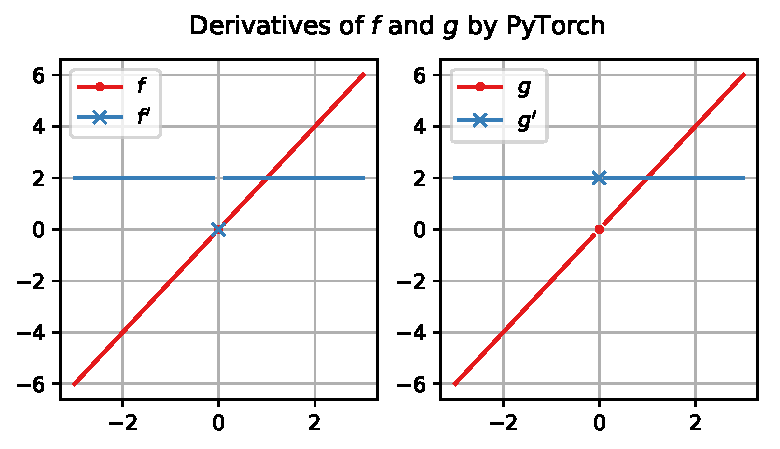
\includegraphics{problem4/problem4_differentiable.pdf}
  \caption{$f$ and $g$ from Listing \ref{lst:fg_diff} plotted along with
    their PyTorch-computed derivatives.}
  \label{fig:problem4_differentiable}
\end{figure}

The code for this exercise can be found at \url{https://gitlab.cs.washington.edu/pmp10/cse547/tree/master/hw1/problem4}.

\section*{Problem 5: Elementary properties of $l_2$ regularized logisitic regression}

\subsection*{The binary case}

Consider minimizing
\begin{equation}
  J(\mathbf{w}) = -l\left(\mathbf{w},\mathcal{D}_\mathrm{train}\right) + \lambda\left\lVert\mathbf{w}\right\rVert_2^2,
\end{equation}
where
\begin{equation}
  l\left(\mathbf{w},\mathcal{D}\right) = \sum_j \log \mathbf{P}\left(
    y^j \mid \mathbf{x}^j, \mathbf{w}
  \right)
\end{equation}
is the log-likelihood on the data set $\mathcal{D}$ for
$y^j \in \{ \pm 1 \}$

State if the following are true or false. Briefly explain your reasoning.

\begin{enumerate}
\item With $\lambda > 0$ and the features $x^j_k$ linearly separable,
  $J\left(\mathbf{w}\right)$ has multiple locally optimal solution.
  \subsubsection*{Solution}
  
  \emph{False}. When the features are linearly separable, we can push loss
  unregularized loss arbitrarily close to $0$ but the the loss is
  still convex. The sum of two convex functions is convex, so there
  will be global optimum.
  
\item Let
  $\hat{\mathbf{w}} = \argmin_{\mathbf{w}} J\left(\mathbf{w}\right)$ be
    a global optimum. $\hat{\mathbf{w}}$ is typically sparse.
    
    \subsubsection*{Solution}
    \emph{False}. This may be true with $l_1$ regularization, but is not
    usually the case with $l_2$ regularization. If one considers the
    dual Lagrangian problem, $\hat{\mathbf{w}}$ will lie on some
    hypersphere at a point which will not generally have $0$ values.
  \item If the training data is linearly separable, then some weights
    $w_j$ might become infinite if $\lambda = 0$.
    \subsubsection*{Solution}

    \emph{True}. By making the weights larger and larger we can push the loss
    to be arbitrarily close to $0$ if $\lambda = 0.$
    
  \item $l\left(\hat{\mathbf{w}}, \mathcal{D}_\mathrm{train}\right)$
    always increases as we increase $\lambda$.
    \subsubsection*{Solution}

    \emph{True}. If one thinks in term of the Lagrangian dual problem
    increasing $\lambda$ is contraining the weights further away from
    the global optimum by restricting them to a smaller hypersphere.

  \item $l\left(\hat{\mathbf{w}}, \mathcal{D}_\mathrm{test}\right)$
    always increases as we increase $\lambda$.
    \subsubsection*{Solution}

    \emph{False}. While the training loss may increase, we could be
    overfitting. Thus, sometimes increasing $\lambda$ may decrease
    test loss.    
\end{enumerate}

\subsection*{Multi-class Logistic Regression}

In multi-class logistic regression, suppose
$Y \in \left\{y_1,\ldots,y_R\right\}$. A simplified version (with no
bias term) is as follows. When $k < R$ the posterior probability is given by:
\begin{equation}
  P\left( Y = y_k \mid X\right) =
  \frac{\exp\left(\left\langle w_k, X\right\rangle\right)}
  {1 + \sum_{j=1}^{R-1}\exp\left(\left\langle w_j, X\right\rangle\right)}.
  \label{eqn:multiclass_log_reg}
\end{equation}

For $k = R$, the posterior is
\begin{equation}
  P\left( Y = y_R \mid X\right) =
  \frac{1}
  {1 + \sum_{j=1}^{R-1}\exp\left(\left\langle w_j, X\right\rangle\right)}.
\end{equation}

To simplify notation, we can define $w_R = \mathbf{0}$ as a vector of
all $0$s. This gives us Equation \ref{eqn:multiclass_log_reg} for all
$k$.

\begin{enumerate}
\item How many parameters do we need to estimate? What are these
  parameters?

  \subsubsection*{Solution}

  Assume the data is $D$-dimensional. Our parameters are the weights
  $w_k$ each which is a $D$-dimensional vector. There are
  $\boxed{(R - 1)D}$ parameters to estimate.
\item Given $N$ training samples
  $\left\{\left(x^1, y^1\right),\left(x^2,
      y^2\right),\ldots,\left(x^N, y^N\right)\right\}$, write down
  explicitly the log-likelihood function and simplify it as much as
  you can:
  \begin{equation}
    L\left(w_1,\ldots,w_{R-1}\right) = \sum_{j=1}^N \log\left(
      P\left(y^j \mid x^j,w\right)
    \right).
    \label{eqn:log_likelihood}
  \end{equation}
  
  \subsubsection*{Solution}

  Let $y^j = y_{l^j}$, that is, let $l^j$ be the class label of observation
  $j$. If we use the posterior probability in Equation
  \ref{eqn:multiclass_log_reg}, then, we have that
  \begin{equation}
    \log\left(
      P\left(y^j \mid x^j,w\right)
    \right)
    = \left\langle w_{l^j}, x^j\right\rangle -
    \log\left(
      1 + \sum_{k=1}^{R - 1}\exp\left(
        \left\langle w_k, x^j\right\rangle
      \right)
    \right).
    \label{eqn:log_p}
  \end{equation}

  Substituting Equation \ref{eqn:log_p} into Equation \ref{eqn:log_likelihood}, we have
  \begin{equation}
    L\left(w_1,\ldots,w_{R-1}\right)
    = \sum_{j=1}^N\left(
      \left\langle w_{l^j}, x^j\right\rangle
      -
      \log\left(
      1 + \sum_{k=1}^{R-1}\exp\left(\left\langle w_k,x^j\right\rangle\right)
      \right)
    \right).
    \label{eqn:log_p_simple}
  \end{equation}
\item Compute the gradient of $L$ with respect to each $w_k$ and simplify it.
  \subsubsection*{Solution}

  $w_k$ is a $D$-dimensional vector so, $\frac{\partial L}{\partial w_k}$ will
  also be $D$-dimensional. Denote the features for the observations with class
  label $k$ by $\mathcal{X}_k = \left\{x^j : l^j = k\right\}$.

  We have that for $k = 1,2,\ldots,R-1$:
  \begin{align}
    \frac{\partial L}{\partial w_k}
    &= \sum_{x \in \mathcal{X}_k} x
      - \sum_{j=1}^Nx^j\frac{
      \exp\left(\left\langle w_k,x^j\right\rangle\right)
      }
      {1 + \sum_{m=1}^{R - 1}\exp\left(\left\langle w_m,x^j\right\rangle\right)}
      \label{eqn:log_likelihood_gradient}\\   
    &= \sum_{x \in \mathcal{X}_k} x -
      \sum_{j=1}^N x^j P\left(Y = y_k \mid X = x^j\right).
      \nonumber
  \end{align}
\item Now add the regularization term $\lambda$ and define a new objective
  function:
  \begin{equation}
    L\left(w_1,\ldots,w_{R-1}\right) = \sum_{j=1}^N\log\left(
      P\left(y^j \mid x^j, w\right)
    \right)
    +
    \frac{\lambda}{2}\sum_{l=1}^{R-1}\left\lVert w_l\right\rVert_2^2.
    \label{eqn:log_likelihood_with_penalty}
  \end{equation}

  Compute the gradient of this new $L$ with respect to each $w_k$.

  \subsubsection*{Solution}

  We can just differentiate term by term. The gradeint of the first term comes
  from Equation \ref{eqn:log_likelihood_gradient}. We can write
  $\left\lVert w_l\right\rVert_2^2 = w_{l1}^2 + w_{l2}^2 + \cdots + w_{lD}^2$,
  so we have that
  \begin{equation}
    \frac{\partial L}{\partial w_l}
    = \sum_{x \in \mathcal{X}_l} x
      - \sum_{j=1}^Nx^j\frac{
      \exp\left(\left\langle w_l,x^j\right\rangle\right)
      }
      {1 + \sum_{m=1}^{R - 1}\exp\left(\left\langle w_m,x^j\right\rangle\right)}
      + \lambda w_l.
  \end{equation}
\end{enumerate}

\end{document}
% Local Variables:
% TeX-command-extra-options: "-shell-escape"
% End: